\section{Grid 1}
\subsection*{题意}
给定一个 $h$ 行 $w$列的网格,现在位于 $(1,1)$,每次可以向下或右走一格,求有多少种方式(对 $10^9 + 7$ 取模)走到 $(h,w)$。

网格中有若干个不能经过的障碍,但不会出现在起点和终点。
\begin{center}
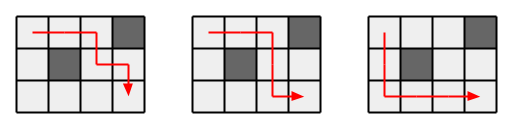
\includegraphics[width=7cm]{Pics/grid.png}
\end{center}
\subsection*{数据范围}
\begin{itemize}
\item $2 \leq h,w \leq 1000$
\end{itemize}
\subsection*{题解}

这题比较简单,用 ${\texttt{dp[i][j]}}$ 表示走到 $(i,j)$ 的方案数,只需要枚举来源即可。转移方程为:
\begin{equation*}
{\texttt{dp[i][j]}} = 
\begin{cases}
 0 & (i,j)\text{ 是障碍}\\
 {\texttt{dp[i-1][j]}} + {\texttt{dp[i][j-1]}} & \text{otherwise}
\end{cases}
\end{equation*}


顺带一提,如果没有障碍,这个 dp 表格就是 \href{https://zh.wikipedia.org/zh-hans/%E6%9D%A8%E8%BE%89%E4%B8%89%E8%A7%92%E5%BD%A2}{杨辉三角},即${\texttt{dp[i][j]}} = {\binom{i+j}{i}}$ 。



\subsection*{核心代码}
\inputminted[linenos,autogobble]{cpp}{../Code/H.cpp}
\newpage